\documentclass{article}
\usepackage{graphicx}
\graphicspath{ {/home/users/jeem9157/} }

\begin{document} 

\title{Summary of Midterm Question 3}
\author{Jeremy Emmett}
\maketitle
In part (a), IDL calculated the value of the specified function of x by calling on the function fx to return the value of f(x). 
\par
In part (b), IDL calculated an approximate value for the integral of the function, given arbitary
bounds of integration, using a Simpson's rule function. 
\par
In part (c), IDL calculated and approximate value for the integral of the function, from x=1 to x=10, using the same Simpson's rule function.
\par
In part (d), IDL calculated the analytical value for the integral of the function, from x=1 to x=10, using an analytical integrator function. The Simpson's rule approximation was found to be 0.003 percent smaller than the analytical value for this integration range. 
\par
The computed values were:
(a)      29.0801
(b)      5.05481
(c)      2526.91
(d)      2527.00
\par
In part (e and f), IDL calculated the accuracy error resulting from splitting the integral into different step sizes. There's a coding issue in using the Simpson's rule function to compute an approximate integral for different step sizes, so the resulting accuracy errors are too large. 
\begin{figure}
\label{figure1}
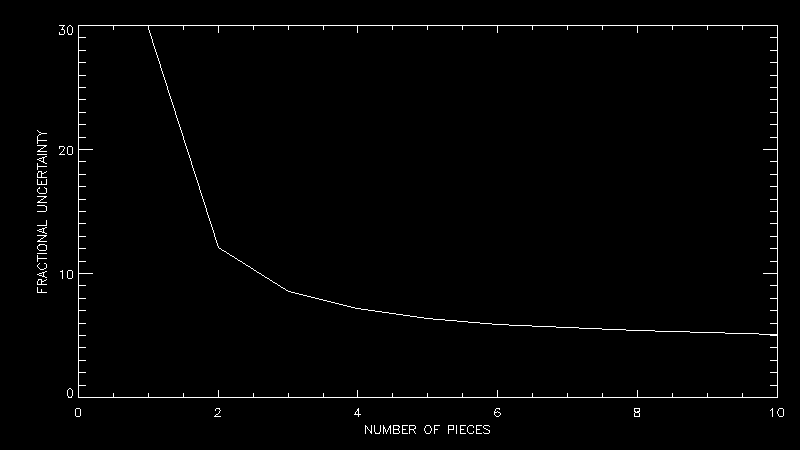
\includegraphics[scale=0.8]{q3png}
\caption{}
\end{figure}

\end{document}
